\documentclass{beamer}

\usepackage{graphicx}

\title{Workflows and Distributed Version Control}

\author{Olof Johansson \& Daniel Persson}

\begin{document}
%    ``When solving problems, dig at the roots instead of just hacking at the leaves.''
\begin{frame}
 \maketitle
\end{frame}

\begin{frame}
 \transwipe
 \frametitle{Agenda}
 \tableofcontents
\end{frame}

\section{Background}
\begin{frame}
 \transwipe
 \frametitle{Background}
 \begin{itemize}
  \item Important tool for software engineers
  \item Useful to ...
  \begin{itemize}
   \item ... keep track of history
   \item ... be able to revert to old versions
   \item ... manage old releases
  \end{itemize}
 \end{itemize}
\end{frame}

\begin{frame}
 \transwipe
 \frametitle{History}
 \begin{itemize}
  \item Local era (RCS, SCCS)
  \item Centralized era (CVS, Subversion, etc)
  \item Distributed era (Mercurial, Git, etc)
 \end{itemize}
\end{frame}

\subsection{Telia Smart Home}
\begin{frame}
 \transdissolve
 \frametitle{Telia Smart Home Context}
 \begin{figure}
  \centering
   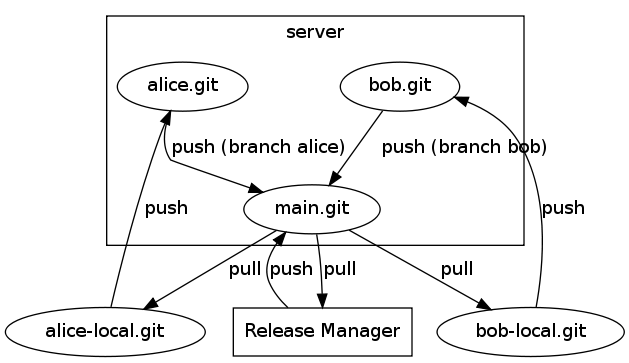
\includegraphics[width=0.7\textwidth]{../workflow} 
  \caption{Workflow employed by the Telia Smart Home project}
 \end{figure}
\end{frame}

\section{Research Design}

\begin{frame}
 \transwipe
 \frametitle{Research Design}
 \begin{itemize}
  \item How does the developers adapt to a distributed workflow?
  \item How does a distributed workflow affect code quality in
        relation to the release management and code review?
 \end{itemize}

 \pause

 \begin{itemize}
  \item Literature Review
  \item Post-Mortem Analysis
   \begin{itemize}
    \item Interviews
    \item Build Metadata
   \end{itemize}
 \end{itemize}
\end{frame}

\section{Findings}
\subsection{Literature Review}
\begin{frame}
 \transwipe
 \frametitle{Migration Costs}
 \begin{itemize}
  \item Increasingly popular
   \begin{itemize}
    \item Perl, Parrot and Curl
   \end{itemize}
  \item Migration of code repositories
  \item Differing nomenclature
  \item Interface differences
 \end{itemize}
\end{frame}

\begin{frame}
 \transwipe
 \frametitle{DVCS Architecture}
 \begin{itemize}
  \item No Enforced Centralization
  \item Offline Work
  \item Performance Benefits
 \end{itemize}
\end{frame}

\begin{frame}[fragile]
 \transwipe
 \frametitle{Quality Implications}
 \begin{itemize}
  \item No Performance Limitations
  \item \verb!bisect!
  \item Code Review
 \end{itemize}
\end{frame}

\subsection{Post-Mortem Analysis}
\begin{frame}
 \transwipe
 \frametitle{Findings from Post-Mortem}
 Internal Survey
 \begin{itemize}
  \item General positive feedback for workflow
  \item High Build Success
  \item Build only broken early in the project
  \item Code Review
  \item Release manager bottleneck
 \end{itemize}

 \pause

 External Survey
 \begin{itemize}
  \item Less than 50\% had previous experience with VCS
  \item Few thought through their VCS workflows
   \begin{itemize}
    \item Those that did described a simple centralized workflow
   \end{itemize}
 \end{itemize}
\end{frame}


\section{Discussion}
\begin{frame}
 \transwipe
 \frametitle{Discussion}
 \begin{itemize}
  \item Migration can be expensive (Perl migration took 22 months)
   \begin{itemize}
    \item An acceptable cost
   \end{itemize}
  \item Personal preferences are important
  \item Performance gain
  \item Flexibility
   \begin{itemize}
    \item Easy to integrate code review or adapt to other workflows
   \end{itemize}
 \item Easier to engage new contributors in open source projects
 \end{itemize}
\end{frame}

\section*{The End}
\begin{frame}
 \transdissolve
 \frametitle{Questions?}
 \begin{quote}
  \begin{center}
   ``Nobody actually creates perfect code the first time around, except me. But there's only one of me.''
  \end{center}
 \end{quote}
 \begin{flushright}
   --- Linus Torvalds, creator of Git.
 \end{flushright}
\end{frame}

\end{document}
